\section[Filtrage par contenu]{Filtrage par contenu}
\subsection{Définition}
\begin{frame}{Définition}
    \begin{itemize}\itemsep1em
        \item[-] Un lac de données (en anglais data lake) est une méthode de stockage des données utilisée par le big data (mégadonnées en français). Ces données sont gardées dans leurs formats originaux ou sont très peu transformées.
        \item[-] Le Data Lake regroupe les données structurées en provenance de bases de données relationnelles en couloir ou en colonne, les données semi-structurées telles que les CSV, les logs, les XML, les JSON, et les données non structurées telles que les emails, les documents et les PDF.
    \end{itemize}
\end{frame}
\begin{frame}{Caractéristique}
    \begin{enumerate}
        \item Un catalogue de métadonnées qui assure la qualité des données
        \item Une politique et des outils de gouvernance  des données
        \item L’ouverture à tous types d'utilisateurs 
        \item L’intégration de données de tous types
        \item Une organisation logique et physique
        \item Le passage à l'échelle.
    \end{enumerate}
\end{frame}

\begin{frame}{Utilisateurs de data lake}
    \begin{figure}
        \centering
        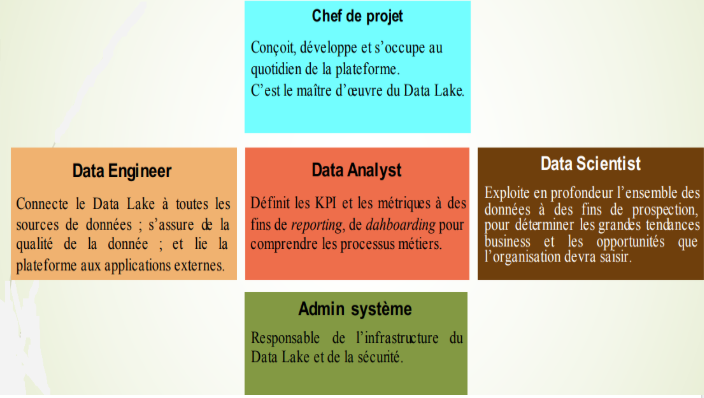
\includegraphics[scale=0.6]{figures/users.PNG}
    \end{figure}
\end{frame}

\begin{frame}{Data lake vs data warehouse}
    \begin{figure}
        \centering
        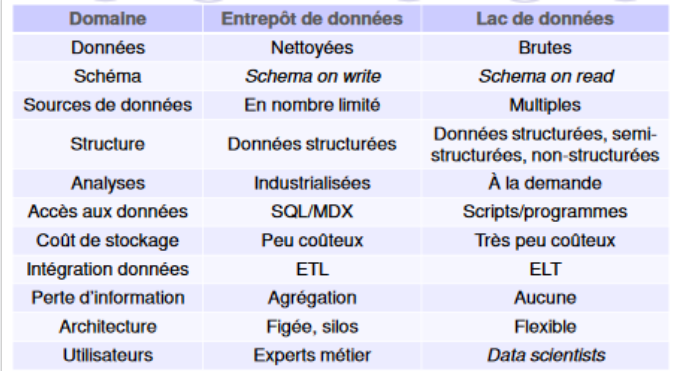
\includegraphics[scale=0.6]{figures/lakevs.PNG}
    \end{figure}
\end{frame}

\subsection{Métadonnées}
\begin{frame}{Métadonnées}
    \begin{itemize}\itemsep1em
        \item \textbf{Métadonnée intra-Objet :}
        \begin{itemize}
            \item[-] Propriétés (nom de fichier, taille, date de création…)
            \item[-] Pré visualisation/résumé (schéma, nuage de mots)
            \item[-] Versions et représentations (Transformation de données)
            \item[-] Métadonnées sémantiques (Description, catégories)
        \end{itemize}
        \item \textbf{Métadonnée inter-Objet :}
        \begin{itemize}
            \item[-] Regroupements (thématique, par langue)
            \item[-] Similarité (Via de mesures de similarité)
            \item[-] Parenté (jointure, unions)
        \end{itemize}
        \item \textbf{Métadonnée globales :}
        \begin{itemize}
            \item[-] Ressources sémantiques( antologie, taxonomie)
            \item[-] Index (y compris index inversés)
            \item[-] Journaux(logs)
        \end{itemize}
    \end{itemize}
\end{frame}

\begin{frame}{Fonctionnalités des système de métadonnées}
    \begin{figure}
        \centering
        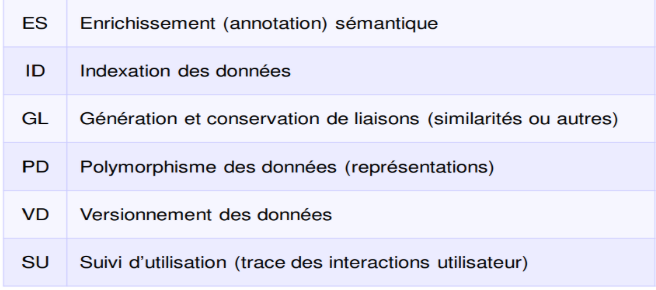
\includegraphics[scale=0.6]{figures/fonctionalite.PNG}
    \end{figure}
\end{frame}

\begin{frame}{Représentation des métadonnées}
   \begin{figure}
       \centering
       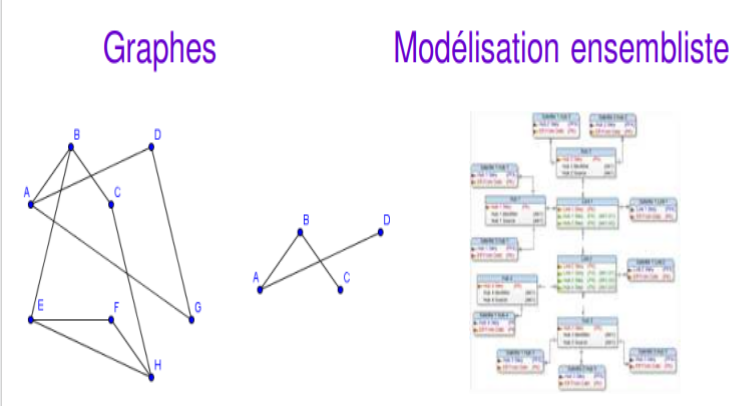
\includegraphics[scale=0.5]{figures/representation2.PNG}
   \end{figure} 
\end{frame}

\begin{frame}{Stockage des métadonnées}
    \begin{itemize}\itemsep1em
        \item \textbf{Orienté document(XML, JSON...)}
        \begin{itemize}
            \item[-] Données structurées et semi-structurées
        \end{itemize}
        \item \textbf{Standards du W3C (RDF, OWL...)}
        \begin{itemize}
            \item[-] Métadonnées sémantiques
            \item[-] Contraintes d’intégrité
        \end{itemize}
        \item \textbf{Base de données (SQL ou NoSQL)}
        \begin{itemize}
            \item[-] Modèles ensemblistes, graphes
            \item[-] Orienté document, clé-valeur
        \end{itemize}
    \end{itemize}
\end{frame}

\subsection{Architecture}
\begin{frame}{Architecture de data lake}
    Il est important de se rappeler qu'un data lake est articulé autour de deux composantes : 
    \vspace{0.2cm}
    \setbeamertemplate{description item}[align left]
    \begin{itemize}
        \item Le stockage 
        \item Le traitement 
    \end{itemize}
    \vspace{0.2cm}
     => Les deux peuvent être effectués sur site ou dans le cloud, d'où de multiples combinaisons possibles lors de la conception d'une architecture de data lake.
\end{frame} 

\subsubsection{Data lakes sur Amazon AWS}
\begin{frame}[allowframebreaks, fragile]{Data lakes sur Amazon AWS}
    \begin{itemize}\itemsep1em
        \item[-] Amazon AWS propose une gamme exhaustive de produits pour sa solution data lake.
        \item[-] Amazon Simple Storage Service (Amazon S3) est au centre de cette solution et assure les fonctionnalités de stockage. Kinesis Streams, Kinesis Firehose, Snowball et Direct Connect sont des outils d'importation de données qui permettent de transférer des volumes considérables de données vers S3. AWS propose également un service de migration de bases de données qui facilite la migration des données du site vers le cloud.

        \item[-] Points forts :
        \begin{enumerate}
            \item Gamme de produits exhaustive et riche en fonctionnalités
            \item Possibilité de sélectionner des produits en fonction de vos besoins spécifiques
            \item Coûts réduits
            \item Normes rigoureuses en matière de sécurité et conformité
            \item La séparation du traitement et du stockage permet de faire évoluer ces opérations en fonction de leurs besoins spécifiques
            \item La collaboration avec des sociétés APN (AWS Partner Network) telles que Talend assure l'intégration transparente des services AWS.
        \end{enumerate}
    \end{itemize}
\end{frame}

\subsubsection{Data lakes sur Hadoop}
\begin{frame}{Data lakes sur Hadoop}
    
    \begin{itemize}\itemsep1em
        \item[-] Un cluster Hadoop de serveurs distribués permet d'apporter une solution pour le stockage des big data. HDFS (Hadoop Distributed File System) – Couche située au cœur de Hadoop et qui assure le stockage et la réplication des données sur plusieurs serveurs. 
        \item[-] Points forts :
        \begin{enumerate}
            \item Déjà connu des spécialistes en technologie
            \item Moins cher parce que open source
            \item Nombreux outils ETL disponibles pour l'intégration avec Hadoop
            \item Évolution facile
            \item La « localité » des données (données et traitement dans le même emplacement) accélère le traitement
        \end{enumerate}
    \end{itemize}
\end{frame}

\subsubsection{Data lake sur Microsoft Azure}
\begin{frame}{Data lake sur Microsoft Azure}
    \begin{itemize}\itemsep1em
        \item[-] Azure est un data lake proposé par Microsoft. Il se compose d'une couche de stockage (Azure Data Lake Store, ADLS) et d'une couche d'analyse constituée de deux éléments : Azure Data Lake Analytics et HDInsight.
        \item[-] Points forts :
        \begin{enumerate}
            \item Le stockage et le traitement dans le cloud simplifient l'administration.
            \item Des services analytiques performants avec des fonctionnalités puissantes
            \item Migration facile à partir d'un cluster Hadoop existant
            \item La plupart des experts en big data connaissent déjà Hadoop et ses outils : il est donc facile de trouver la main d'œuvre qualifiée requise
            \item Grâce à l'intégration avec Active Directory, il n'est pas nécessaire de prévoir d'opérations distinctes pour gérer la sécurité.
        \end{enumerate}
    \end{itemize}
\end{frame}
